\subsection{Udvikling}
Formålet med dette afsnit er at give en beskrivelse af programmets opbygning og struktur, samt ved brug af kodeeksempler og teori beskrevet i \ref{sec:teori} at forklare hvordan funktionerne i programmet virker og hvad de gør. I afsnittet vil der være kodeeksempler på prototyperne til funktionerne og kodeeksempler på selve funktionen. Hele programmet kan findes i bilag XX.

\subsubsection{Datastrukturer}
[Indledning: Forklar at vi bruger datastrukturer for at abstrahere over data.]
\paragraph{Vektor}
En stor del af opgaven bygger på vektorer i rummet. Nedenstående kodeuddrag viser hvordan der er abstraheret over en vektor i programmet. 

\begin{lstlisting}[style=Cstyle, caption=Struct til vektor]
typedef struct _vector {
    double x, y, z;
} Vector;
\end{lstlisting}

På linje 2 i ovenstående kodeuddrag er det vist hvordan en 3D vektors koordinarter er beskrevet med typen double. 

\paragraph{Stråle}
For at benytte sig af ray-tracingmetoden er det naturligvis nødvendigt at have en ray (stråle) som man kan trace (følge). 

\begin{lstlisting}[style=Cstyle, caption=Struct til ray]
typedef struct _ray {
  Vector initial_point, direction;
} Ray;
\end{lstlisting}

På linje to i ovenstående kodeuddrag kan det ses at en ray består af et startpunkt (initial_point) og en retning, begge af disse er af typen Vector, som tidligere er beskrevet til at have et x-, y- og z-koordinat.

\paragraph{Trekant}
Enhver figur i programmet består af mange sammensatte trekanter. I de fleste tilfælde er det så mange trekanter, at det ikke umiddelbart er synligt for det blotte øje. Et hjørne i en trekant udspændes af flere og kaldes en vertex.
    
\begin{lstlisting}[style=Cstyle, caption=Struct til vertex]
typedef struct _verticie {
  Vector position;
  Vector normal;
} Vertex;
\end{lstlisting}

På linje to og tre i ovenstående kodeuddrag kan det ses at en vertex består af et stedvektor, som er kaldet position, og en normalvektor.
    
Som nævnt for ovenstående struct for en vertex, er alle objekter i programmet bestående af trekanter. Nedenstående kodeuddrag viser hvordan trekanter er implementeret i programmet.
    
\begin{lstlisting}[style=Cstyle, caption=Struct til triangle]
typedef struct _triangle {
  Vertex *verticies[3];
  Vector edges[3];
} Triangle;
\end{lstlisting}

Denne struct viser, kort sagt, at en trekant består af tre hjørner, altså tre verticies, af typen Vertex, samt tre edges, der er stedvektorer til de tre verticies.

\paragraph{Point\_lights}

En raytracers formål er at følge lysstrålerne, som udskydes fra et bestemt punkt, som i vores tilfælde er fra en pære. 

\begin{lstlisting}[style=Cstyle, caption=Struct til light]
typedef struct _pointlight {
  Vector position;
  Pixel color;
  double intensity;
  double radius;
  int sampling_rate;
} PointLight;
\end{lstlisting}

På linje to i ovenstående kodeuddrag kan det ses, at et lys har en given position, som bestemmes af ét 3D-koordinat. Dette lys har en farve, bestående af en RGB-værdi. Derudover har lyset også en intensitet og radius af typen double, samt sampling_rate af typen int.

\paragraph{Materiale}
I virkeligheden har vi mange forskellige materialer der både syner og føles anderledes end andre. En helt ny bil skinner når man lyser på den, mens en murstensvæg er helt mat. For at illustrere det i raytracing har vi brugt nogen værdier der ofte bruges i forbindelse med 3D-rendering og især raytracing. Vi har valgt at bruge Phong-modellen da den er relativ simpel og giver et godt resultat.

\begin{lstlisting}[style=Cstyle, caption=Struct til Material]
typedef struct _material {
  double ambient_coefficient;
  double diffuse_coefficient;
  double specular_coefficient;
  int smoothness;
  double metalness; 
} Material;
\end{lstlisting}

Ambient_coefficient er værdien der fortæller hvor lyst objektet er selvom der ikke er direkte lys på den. Den bevirker at hvis objektet er i skygge så er det ikke helt sort.
Diffuse_coefficient er skygge-værdien der viser hvor stor indflydelse lys har på objektet. 
Specular_coefficient er værdien der viser hvor meget objektet spejler igen. Denne værdi er høj for en ny poleret bil, men næsten 0 hvis det er en murstensvæg. I vores program gør det at vi får en næsten hvid plet hvis vores lyskilde spejler igen.

\paragraph{AABB}
AABB står for axis aligned bounding boxes, og er en kasse hvis sidder er parallelle med akserne. En boks består af to vektorer som indeholder det laveste og største koordinatsæt for boksen. De to vektorer er en stedvektor til det hjørne på boksen som er tættest på og længst væk fra origo. Nedenstående kodeuddrag viser hvordan dette er gjort i programmet.

\begin{lstlisting}[style=Cstyle, caption=Struct til bounding boxes]
typedef struct _plane {
  Vector low, high;
\end{lstlisting}

De to punkter til boksen er angivet som stedvektorer af typen vector (linje 2).

\paragraph{Plan}
Et plan i rummet er beskrev ved et punkt og en normalvektor til planen. Hvordan dette er gjort i programmet er vist i nedenstående kodeuddrag. 

\begin{lstlisting}[style=Cstyle, caption=Struct til plan]
typedef struct _plane {
  Vector normal;
  Vector point;
\end{lstlisting}

Planens normalvektor er beskrevet med typen vector (linje to). Et punkt til planen er angivet som en stedvektor af typen vector (linje tre).

\paragraph{Skæring}
Det er nødvendigt at vide, hvis og hvor en lysstråle skærer et objekt, for at finde de data (farve, materiale, lokation m.m.) der er i det givne punkt ved skæringen.

\begin{lstlisting}[style=Cstyle, caption=Struct til intersection]
typedef struct _intersection {
  Vector normal;
  Material material;
  Pixel color;
  Triangle *triangle;
  Ray ray;
  double t;
} Intersection;
\end{lstlisting}

På ovenstående struct kan det ses, at hver intersection har en mængde data, som bruges senere til phong. Hver intersection har en 
normalvektor, et materiale, en farve beskrevet ved typen Pixel. Den har derudover en 'triangle' til at finde hvilken trekant i træet, som den skærer i, en 'ray', som beskriver lysstrålen, der skærer i det givne punkt samt en tid t af typen double, der beskriver afstanden fra initialpoint.

\paragraph{Billede}
Vi har en Image-struct for at simplificerer måden vi udskriver pixels på og forbedre læseligheden.

\begin{lstlisting}[style=Cstyle, caption=Struct til Image]
typedef struct _image {
  unsigned int width, height;
  Pixel **pixels;
} Image;
\end{lstlisting}

Vores Image-struct definerer 2 doubles der beskriver højden og bredden på vores billede i pixels.
Vi har også et 2-dimensionelt array med Pixels der beskriver vores billede.

\paragraph{Kamera}
Som vist på figur \ref{...} i afsnit \ref{...} er kameraet beskrevet som dens position og orientering i rummet samt en afstand, d, til kameraet. Derudover har kameraet en højde og en bredde som definerer billedets opløsning. Nedenstående kodeuddrag viser hvordan dette er gjort i programmet.

\begin{lstlisting}[style=Cstyle, caption=Struct til kamera]
typedef struct _camera {
  Vector up;
  Vector right;
  Vector forward;
  Vector position;
  unsigned int width, height;
  double distance;
} Camera;
\end{lstlisting}

Kameraets orientering kan beskrives som tre vektorer af typen vector (linje 2-4). Kameraets position kan angives som en stedvektor af typen vector (linje 5). Opløsningen er angivet som positive heltal af typen unsigned int (linje 6). Afstanden til kameraet er angivet som typen double (linje 7).

\paragraph{Scene}
Scenen er den virtuelle verden, som skal visualiseres. I programmet er scenen beskrevet på følgende måde. 

\begin{lstlisting}[style=Cstyle, caption=Struct til scene]
typedef struct _scene {
  Object **objects;
  unsigned int n_objects;
  PointLight **lights;
  unsigned int n_lights;
  Pixel ambient_intensity;
} Scene; 
\end{lstlisting}

En scene består af en række objekter (linje 2-3), en række lys (linje 4-5), samt den ambiente lys intensitet der bruges i Phong.

\paragraph{Objekt}
Objektet er det man kan se når billedet bliver renderet af raytraceren. I programmet er objektet beskrevet på følgende måde.

\begin{lstlisting}[style=Cstyle, caption=Structs til objektet]
typedef struct _object {
  Vertex *verticies;
  int n_verticies;
  Triangle *triangles;
  int n_triangles;
  Pixel color;
  Material material;
} Object;
\end{lstlisting}

Et objekt består af en række verticies (linje 2-3), en række trekanter (linje 4-5), samt en farve på objektet og koefficienterne til det materiale den er lavet af.
\paragraph{K-dimensionalt træ}
Da programmet er bygget op efter at skulle kunne implementeres på en hjemmeside, er renderingen nødt til at være hurtigt. Dette opnås ved hjælp af optimering, hvor der i programmet er brugt KD-træer.

\begin{lstlisting}[style=Cstyle, caption=Struct til KDNode]
typedef struct _KDNode {
  struct _KDNode *low, *high;
  AABB box;
  Triangle **triangles;
  int n_triangles;
} KDNode;
\end{lstlisting}

Et KD-træ består af en række nodes (linje 2), hvilket er forgreninger, den består af en AABB box (linje 3) og en række trekanter (linje 4-5).

\subsubsection{Overordnet programstruktur}
Main funktionen er den funktion som fortæller computerens operativ system hvilke kommandoer den skal udføre. Det er således i funktionen main, at programmets funktioner kaldes og eksekveres. Programmets main funktion er vist nedenfor:

\begin{lstlisting}[style=Cstyle, caption=Main]
int main(int argc, char* argv[]) {
  Scene *scene;
  Camera *camera;
  Image *image;
  Configuration conf;

  unsigned long t0 = time(NULL);
  conf = create_configuration();
  
  if(input_parse(argc, argv, &scene, &camera, &conf) == 0) {
    return -1;
  }
  
  image = raytracer_render(scene, camera);
  
  image_write(image, conf.out_file);

  free_camera(camera);
  free_scene(scene);
  
  printf("%lus\n", time(NULL) - t0);
  return 0;
}
\end{lstlisting}

På linje 1 i ovenstående kodeuddrag, kaldes main, med parametrene argc og argv. argv indeholder en liste af programparametre som f.eks.\ favetemperaturen som ønskes anvendt af programmet. argc er blot antallet af programparametre som argv indeholder. På linje 10 behandles program parametrene og der testes om der er fejl i inputet, hvilket kunne være en manglende 3D-model. Dette gøres gennem input\_parse-funktionen i input.c. På Linje 14 kaldes funktionen raytracer\_render som renderer billedet. Linje 7 og 21 bruges udelukkende til teknisk anvendelse, for at kunne se hvor lang tid programmet har taget om at fuldføre.

\paragraph{Input}
Som input kræver programmet filnavnet på en 3D-model i PLY formatet, derudover modtager programmet en række valgfrie input parametre:
\begin{itemize}
  \item -h [INT]: Et heltal som angiver højden af det resulterende billede i pixel
  \item -w [INT]: Et heltal som angiver breden af det resulterende billede i pixel
  \item -t [INT]: Et heltal som angiver farvetemperaturen af lyskilder i modellen hvis farve er angivet som sort
  \item -H [FLOAT]: Et decimaltal som angiver, i radianer, en horisontal rotation om en sort lyskilde
  \item -V [FLOAT]: Et decimaltal som angiver, i radianer, en vertikal rotation om en sort lyskilde
  \item -o [STRING]: En tekststreng som angiver placering og navnet på det resulterende billede
\end{itemize}

Input 3D-modellen skal være det første programparameter og skal være i et tilpasset PLY format. Data input har ikke været fokuset for opgaven og et tilpasset PLY var blot den nemmeste måde, hurtigt at få et system op at køre så der kunne udvikles forskællige modeller til test. Af samme grund har input parseren heller ikke været et fokus.

\subsubsection{Beskrivelse af raytracer}
[Indledning]
\paragraph{Rendering}
For at rendere et billede af lampen og dens belysning, er der lavet en funktion raytracer\_render, der modtager scenen, dvs. samlingen af alle 3D-objekter og lys, samt modellen for det kamera, som billedet skal dannes ud fra. Funktionen er vist herunder.

\begin{lstlisting}[style=Cstyle, caption=Funktionen der rendere billedet af scenen med et kameras perspektiv]
Image *raytracer_render(Scene *scene, Camera *camera) {
  int x, y;
  Image *image;
  Ray ray;

  image = new_image(camera->width, camera->height);
  
  /* For each column: */
  for(x = 0; x < camera->width; x++) {
    /* For each pixel in column: */
    for(y = 0; y < camera->height; y++) {
      /* Calculate ray */
      ray = raytracer_calculate_ray(x, y, camera);
      
      /* Trace ray and assign result to pixel */
      image->pixels[x][y] = raytracer_trace(ray, scene);
    }
    printf("%.1f\n", ((double)x + 1) / camera->width * 100);
  }

  return image;
}
\end{lstlisting}

Funktionen vist herover, danner en lysstråle for hver pixel i billedet. lysstråle sendes videre sammen med scenen til funktionen raytracer\_trace, som returnere hvilken farve den pågældende pixel på billedet skal have. Til sidst returneres så det endelige billede.

\paragraph{Tracer}
Funktionen raytracer\_trace er den funktion som starter raytraceren samt returnerer en pixelfarve hvis en ray skærer med et objekt i scenen. Funktionen er vist herunder.  

\begin{lstlisting} 
Pixel raytracer_trace(Ray ray, Scene *scene) {
  Intersection intersection = create_intersection();
  Pixel pixel = {0, 0, 0};
  
  /* If ray intersects with scene: */
  if(raytracer_scene_intersection(ray, scene, &intersection)) {
    /* Shade pixel */
    pixel = raytracer_phong(intersection, scene);
  }
  
  return pixel;
}
\end{lstlisting}
Funktionen initialiserer en skæring med værdien -1 ved at kalde funktionen create_intersection (linje 2), og en pixel initialiseres til at indeholde RGB-værdien for farven sort (linje 3). Der checkes efterfølgende om den pågældende ray skærer med et objekt i scenen (linje 6), hvis den gør det så tildeles der en RGB-værdi (linje 8), som returneres til sidst i funktionen. 

\paragraph{Skæring med scene}

Funktionen raytracer\_scene\_intersection tjekker om en ray skærer med et objekt.

\begin{lstlisting}[style=Cstyle, caption=Structs til objektet]
int raytracer_scene_intersection(Ray ray, Scene *scene, 
                                 Intersection *intersection) {
  int i;
  Intersection temporary_intersection;

  temporary_intersection = create_intersection();

  /* For each object in scene: */
  for(i = 0; i < scene->n_objects; i++) {
    /* If ray intersects with object: */
    if(raytracer_object_intersection(ray, scene->objects[i], 
       &temporary_intersection))
      /* Reassign intersection if current intersection is closer */
      if(temporary_intersection.t < intersection->t || intersection->t == -1)
        *intersection = temporary_intersection;
  }
  return intersection->t > 0;
}
\end{lstlisting}

If-sætningen på linje 11 assigner temporary\_intersection til en intersection hvis rayen rammer et objekt. If-sætningen på linje 14 sørger for at det er den intersection der er tættest på der bliver sendt tilbage. 


\paragraph{Skæring med objekt}

\paragraph{Skæring med KD-træ}

\paragraph{Skæring med trekant}

\paragraph{Phong pixel farve}





\subsubsection*{Opsummering}

I afsnittet er der, ved brug af kodeeksempler, blevet dokumenteret for hvordan programmet er udviklet. Vi forventer nu at programmet kan:

\begin{enumerate}
    \item Modtage input fra brugeren heraf en 3D-fil, billedets opløsning, en farvetemperatur for pæren og en kameraposition.
    \item Rendere et billede ud fra den angivne input
    \item Gemme billedet
\end{enumerate}

Nedenstående figur viser en rendering foretaget af det færdige program. 

\begin{figure}[H]
    \centering
    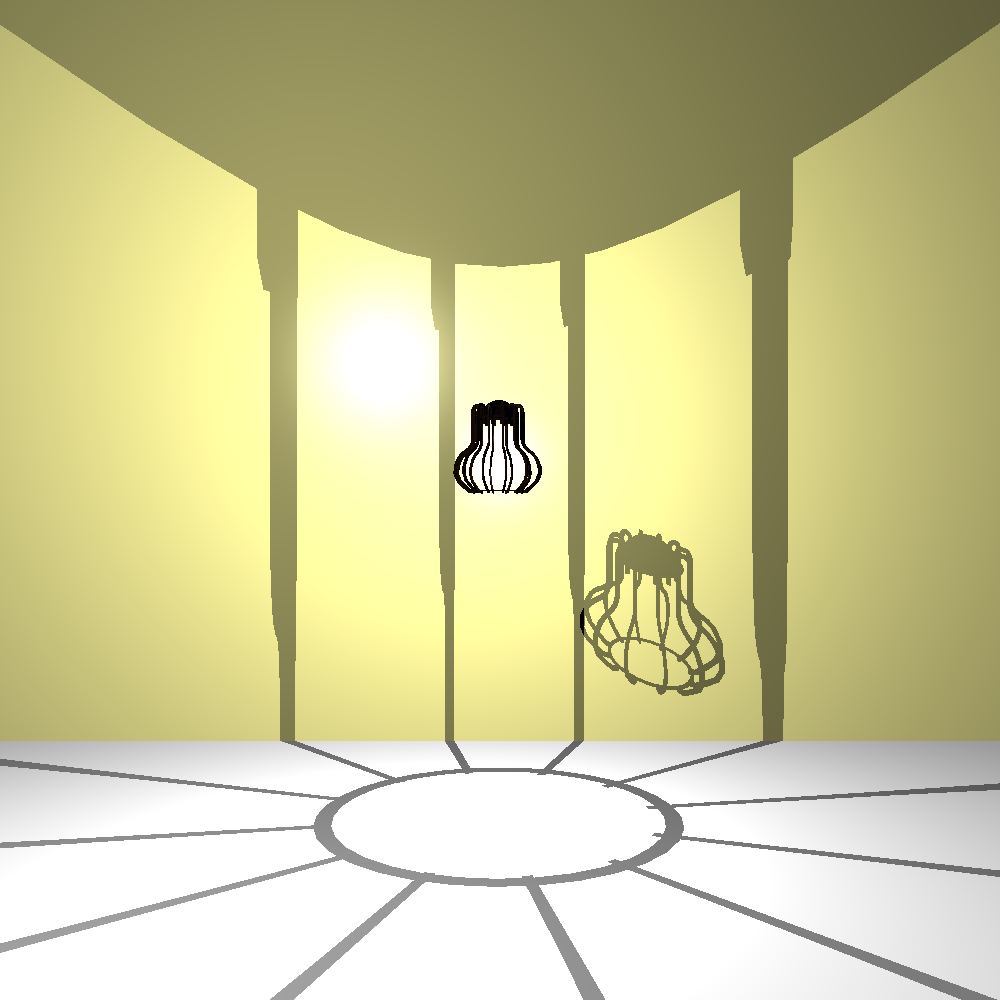
\includegraphics[width=5cm]{skeletonlamp}
    \caption{Eksempel af en rendering fra det færdige program.}
\end{figure}
